\documentclass[12pt, a4paper]{article}

\title{\textsc{Logic Design} Lab 3: \textsf{\Large Pattern Matching} Report}
\author{110062219}
\date{\today}

\usepackage{amsmath}
\usepackage{amssymb}
\usepackage{caption}
\usepackage{subcaption}
\usepackage{circuitikz}
\usepackage{karnaugh-map}
\usepackage{float}
\usepackage{listings}
\usepackage{tikz}
\usetikzlibrary{graphs}
\usetikzlibrary{calc}

\begin{document}

\maketitle

\section{Design of Finite State Machine}

We are to carry out a patter matching module for a certain sequence of binary sequences in the Lab 3. The pattern is described like a \textsf{regular expression}: \textsf{010(101)+11}, which is equivalent to \textsf{010101(101)*11}.

On top of the \textsf{regex}, we could derive the \textbf{Nondeterministic Finite Automata (NFA)} and \textbf{Deterministic Finite Automata (DFA)}. By reducing redundant states, we could obtain the state diagram (Figure \ref{sd}).

The forward edges could be constructed by the definition. Since we accept none or more \texttt{101} in the middle, we have a loop from the last \texttt{1} to the first \texttt{1}. The backward edges are far more difficult. When we fail to match, we should go back to the \textsf{LPS}, i.e. the longest prefix which is also a suffix of current state. I'll explain more details later.

\begin{table}[htbp]
\centering
\begin{tabular}{c|c|c|c|c}
State & 0 & 1 & Output & \textsf{LPS} when unmatched \\
\hline
A0 & B1 & A0 & 0 & \texttt{""} \\
B1 & B1 & C2 & 0 & \texttt{"0"} \\
C2 & D3 & A0 & 0 & \texttt{""} \\
D3 & B1 & E4 & 0 & \texttt{"0"} \\
E4 & F5 & A0 & 0 & \texttt{""} \\
F5 & B1 & G6 & 0 & \texttt{"0"} \\
G6 & F5 & H7 & 0 & \texttt{"01010"} \\
H7 & J9 & I8 & 0 & N/A \\
I8 & B1 & A0 & 1 & \texttt{"0"} \\
J9 & B1 & K10 & 0 & \texttt{"0"} \\
K10 & D3 & H7 & 0 & \texttt{"010"} \\
\end{tabular}
\caption[]{State Table\footnotemark}
\label{st}
\end{table}

\footnotetext{The states are named by a letter and a digit so that we could refer them by either.}

\begin{figure}[htbp]
\centering
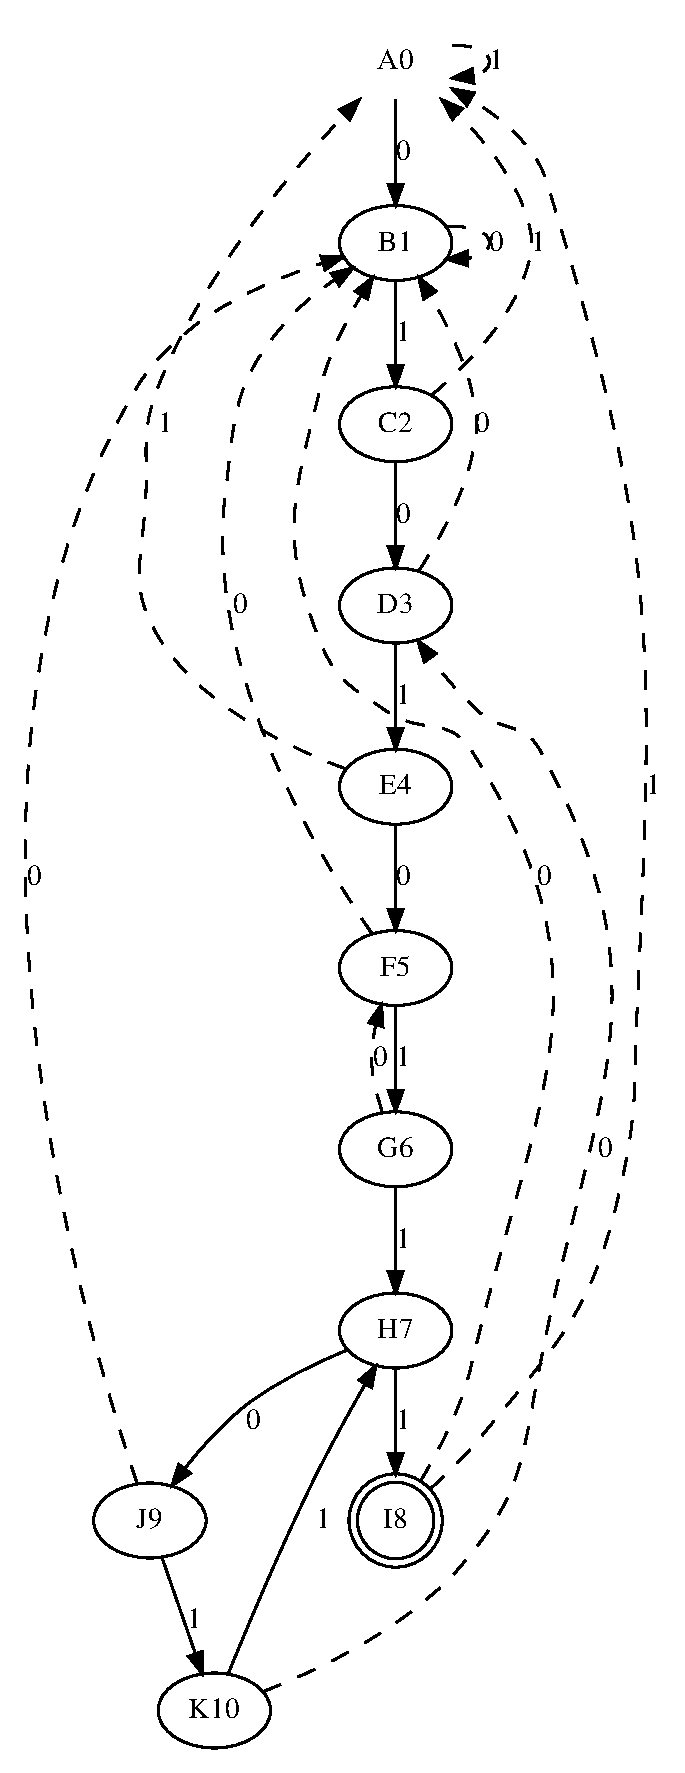
\includegraphics[scale=.69]{states}
\caption{State Diagram}
\label{sd}
\end{figure}

\section{Implementation in \texttt{verilog}}

The 11 states are declared as \texttt{parameter}s. We need two 4-bit registers to record current state and next state.
\lstinputlisting[language=verilog, linerange={6-7}, breaklines=true, tabsize=4]{../src/PAT.v}

Our \textbf{Moore Machine} consists of 3 parts: the next state logic (combinational, synchronous circuit), the output logic and the current state register (sequential, asynchronous circuit).

\subsection{Next State Logic}

I made use of \texttt{case}-block and ternary conditional operator so that my codes are quite concise and make sense.

\lstinputlisting[language=verilog, linerange={9-25}, tabsize=4]{../src/PAT.v}

\subsection{Output Logic}

There's no need to declare the \texttt{flag} as a register and utilize an \texttt{always}-block. It's enough to assign it as a wire with simple logic expression.

\lstinputlisting[language=verilog, linerange={27-27}, tabsize=4]{../src/PAT.v}

\subsection{Current State Register}

The transition of the states takes place when the positive clock edge occurs. If \texttt{reset}, the state goes back to $A$.

\lstinputlisting[language=verilog, linerange={29-33}, tabsize=4]{../src/PAT.v}

\section{Problems}

This time, I also encountered several problems without exception to previous labs.

\subsection{Accept Input Prematurely}

Initially, I designed the \textbf{FSM} as \textbf{Mealy Machine} and didn't have the state $I$. Instead, I directly connected state $H$ to state $A$ with a 1/1 edge and to state $B$ with a 0/0 edge. The output \texttt{flag} was assigned to \texttt{!reset \&\& state == H \&\& data} then.

Nonetheless, my module failed to the test case 0 and mismatched the sequence like \texttt{0101011}. I took a look at the wave shown in Figure \ref{ww}, realizing that the problem is due to time difference.

\begin{figure}[htbp]
\centering
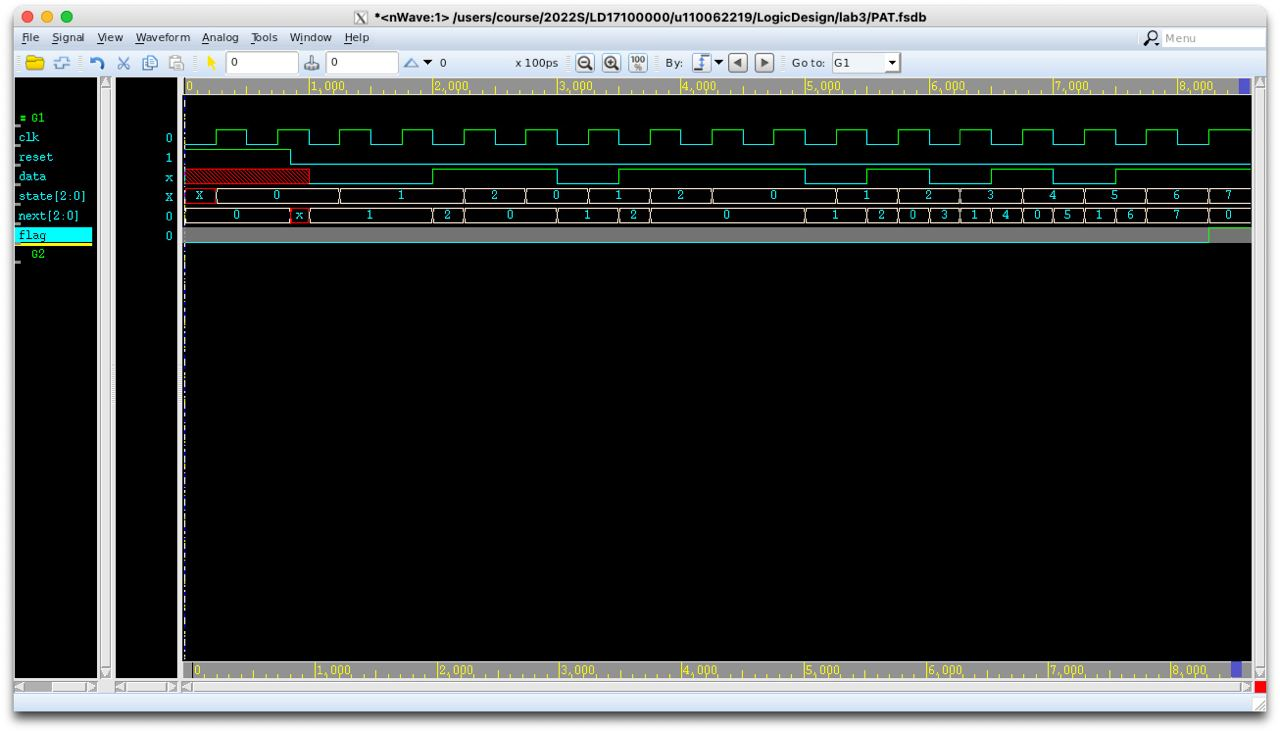
\includegraphics[width=.85\textwidth]{wrong_wave.jpg}
\caption{Wrong Wave}
\label{ww}
\end{figure}

When the current state was $H$, the output is \textsf{true} if the next input is 1. But in my original design, the output would be \textsf{true} right at state $H$ since it catch the current input.

As a consequence, I added the state $I$. Thus, the output depends on  current state only and never triggers too early again. That is, my \textbf{FSM} became \textbf{Moore Machine}.

\subsection{Wrong Backward Edges \& State Reduction}

I didn't come up with the whole state diagram at a time. In fact, I even just found some mistakes while I was writing this report, one of which is I connected state $E$ to state $C$ when unmatched. Interesting enough, these didn't affect that I passed all 3 test cases of both simulation and synthesis.

The longest time I struggled on was the backward edge of state $G$. At first I connect that to state $B$ but failed at line 32 of test case 1. I checked again and connect it to state $D$. However, I failed again at line 75 of test case 1. So I pondered for a while and connect it to state $F$. Subsequently, I passed the remaining test cases of both simulation and synthesis.

Though, I'm really afraid that I still have some mistake. I discussed with my friend and found another fatal flaw in my design. I used to interpret the \textsf{regex} directly and connected state $H$ back to state $F$ if the input is \textsf{false} to form a loop. Nevertheless, there were a problem hidden. When we were at the \texttt{0} in the \texttt{101} (state $G$) and failed to match, the \textsf{LPS} was different depending on whether it was our first time to visit. That's why I used to connect it to state $D$ in the previous paragraph. Thus, I reinterpreted the \textsf{regex} as \textsf{010101(101)*11}, adding two more states to separate the first and further visits. It seemed that I reduced these two state in the very beginning, regarding $J$, $K$ as equivalent to $F$, $G$ respectively.

% Hope I don't miss anything anymore.

\section{Reflections \& Questions}

This lab is quite intriguing for me. I wasn't very concentrated on the courses until Prof. Mak lectured on the example 5 of sequential circuit, which was pattern recognizer. It raised my interest immediately since I learnt some algorithm about string matching such as \textbf{Knuth-Morris-Pratt (KMP)} and \textbf{Gusfield (Z)} before.

The crucial key to pattern matching is to construct those backward edges when unmatched. This has a lot to do with \textsf{Failure Function} in \textbf{KMP}. So how to find it? We need to find the \textsf{LPS}, i.e. the longest proper prefix, which is also a suffix of current state, which is what \textbf{Z} does.

I also have some questions to ask TAs:

\begin{itemize}
\item Could this lab be done in \textbf{Mealy Machine}? If so, how to avoid the situation I ran into in \textbf{Section 3.1}?
\item In what circumstance one module would pass the simulation but fail the synthesis? I don't know the meaning to use the Digital Vision.
\item It seems that \texttt{verilog} is such a high-level \textbf{HDL} that we needn't deal with those bothersome latches or flip-flops at all.  Are they, along with muxs, decoders and so forth, really important?
\item Could you release more hard test cases? I passed all of them while having two flaws.
\item Could we have our second midterm paper back? Will the final exam be taken physically?
\item Will the professor kindly ``curve'' our grades? I didn't do so well in the two midterms though having such fun time doing all three labs. Nonetheless, I'm quite anxious about my grade.
\end{itemize}

\end{document}
